\section{Role of energy storage - a survey}
\label{ch-literature:sec:role-of-energy-storage-a-survey}


\begin{figure}\centering
	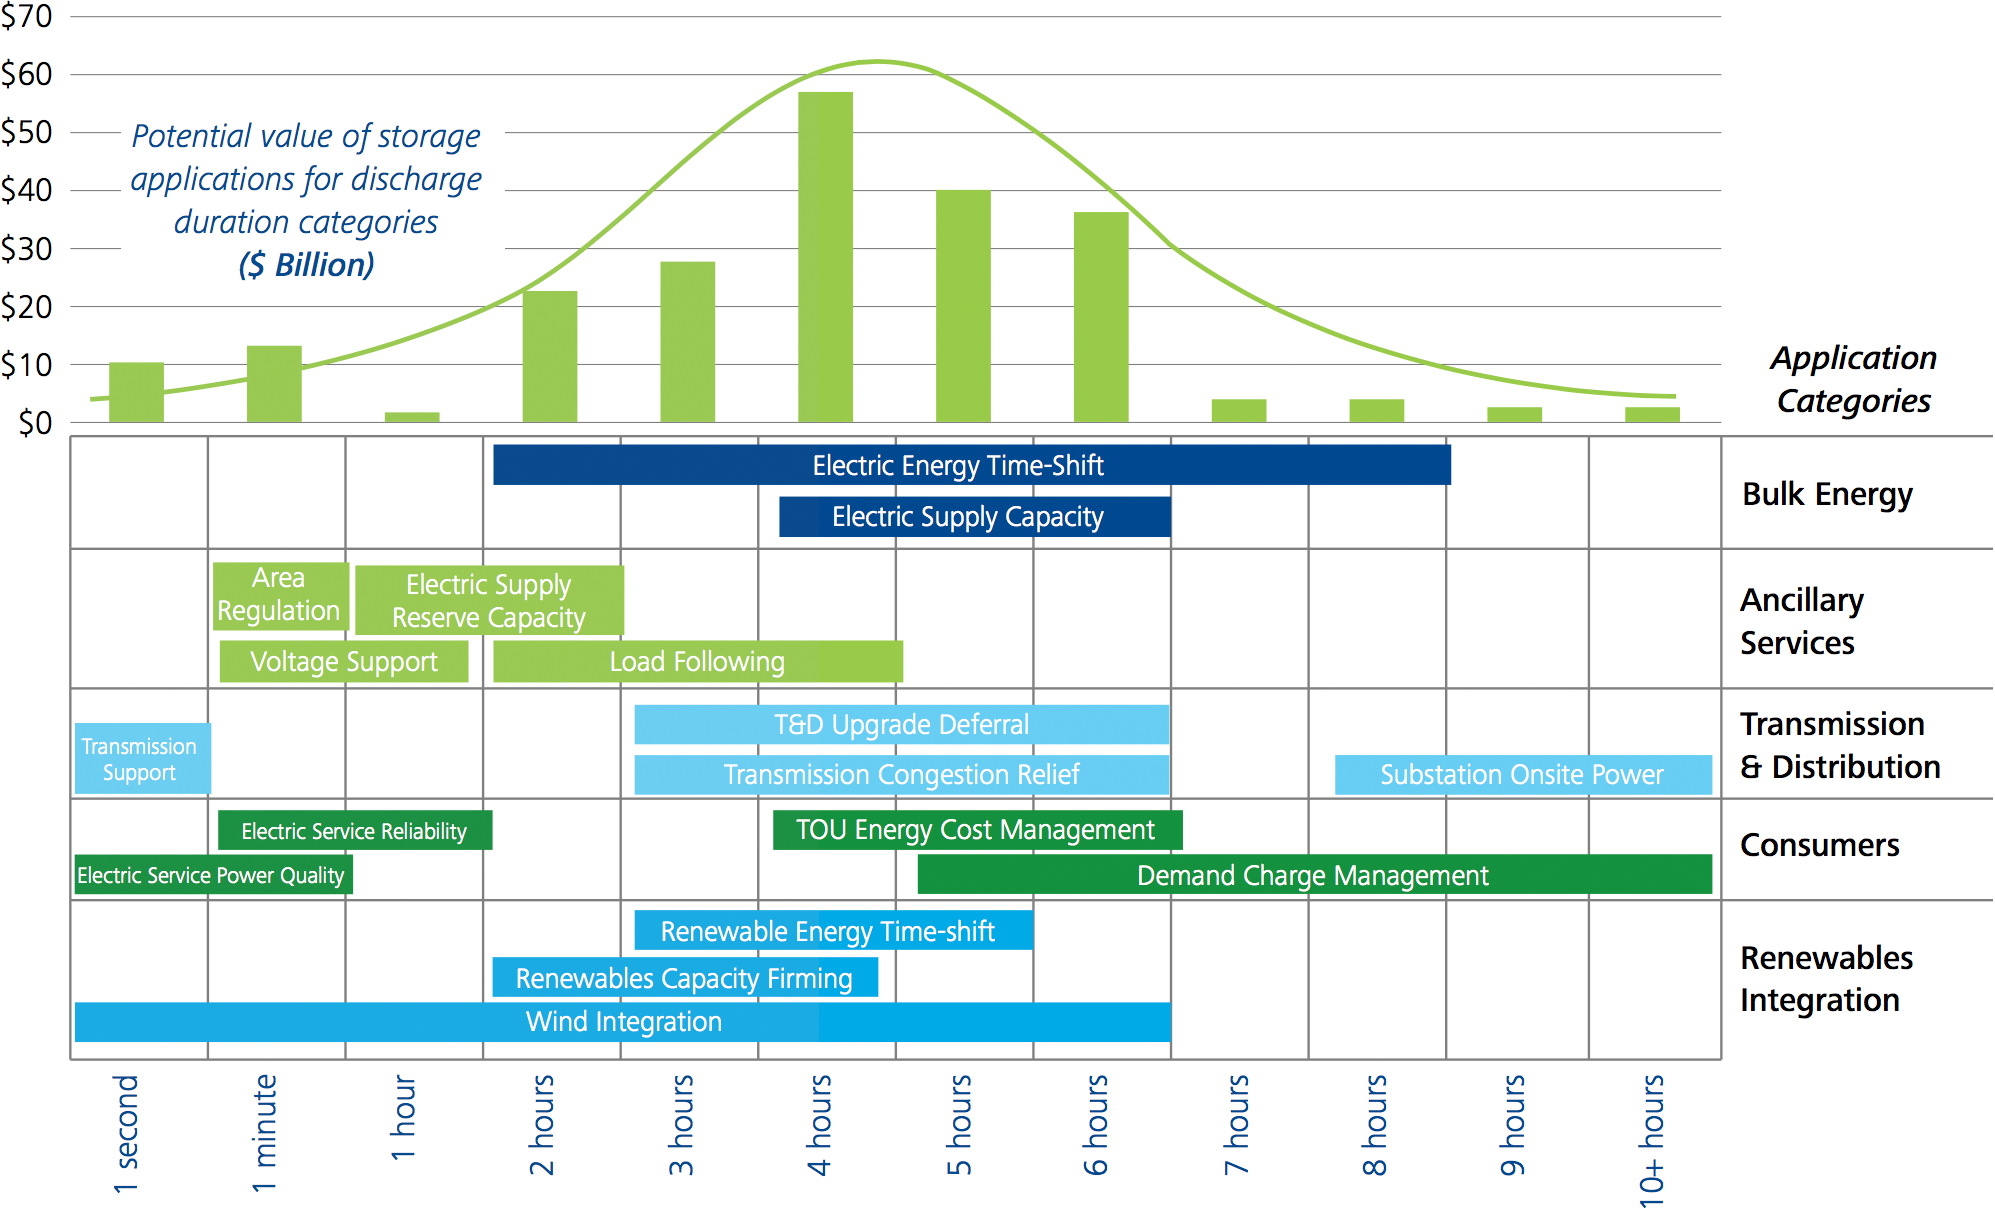
\includegraphics[width=\textwidth]{_literature/fig/storage-financial-benefits}
	\caption{Energy storage applications and corresponding value for various discharge durations \cite{Deloitte2016}}
	\label{ch-literature:fig:storage-financial-benefits}
\end{figure}

The idea of using energy storage in the electricity grid has been discussed for quite some time, and its important role in future energy systems has already been identified in the 70s \cite{Kalhammer1979}.
As the name suggests, electrical energy storage systems have the ability to both consume, store, and release electrical energy by converting it into a different form of energy.
Depending on the rate at which energy can be consumed and released, i.e. the system's power, as well as the amount of energy that can be stored, i.e. system's capacity, different functions can be provided.
A study for the Department Of Energy (DOE) showed that, when correctly exploited, these functions can yield direct financial benefits of \$157.56 billion over an estimated 10 year system lifecycle \cite{Eyer2010a}.
Figure \ref{ch-literature:fig:storage-financial-benefits} shows these benefits in relation to the storage system's typical discharge period, and links them to their associated functions, too.
Here, Time Of Use (TOU) energy cost management yields the largest economic profit, yet from a historical point of view, bulk energy storage has played the most important role in the energy system.

Nowadays, storage can also tap into emerging revenue streams and perform additional functions.
As identified in several review articles \cite{Chen2009, Katsanevakis2017, Guney2017}, the key roles and applications of energy storage systems, regardless of profitability in the current market situation, can be identified as follows:

\begin{itemize}
\item
\textbf{Energy shifting - arbitrage}: This function uses the difference in energy price to yield revenue.
More specifically, as energy pricing is expected to become more dynamic and responsive to current energy demand and generation, storage is controlled to charge when energy prices are low and discharge when energy prices are high \cite{Chen2009, Leou2012}.
Such dynamic pricing schemes are expected to emerge due to significant changes in demand at morning and evening peaks \cite{Koohi-Kamali2013}.
\item
\textbf{Supply capacity}: In order to meet future energy demand, energy suppliers commit their resources in advance.
Doing so allows them to plan for their operation and solve the economic dispatch problem.
With increasing demand, the supply volume will have to increase, too.
However, it is predicted that energy storage can defer or even avoid investments in power plants, assuming they are sized accrodingly (i.e. several 100MW)\cite{Dobie1998}.
Bulk energy storage was the first choice to support supply capacity.
One example is pumped hydro-electric energy storage, which has seen a global growth of 127GW since 1979 \cite{Rehman2015, Barbour2015, Barbour2016}.
\item
\textbf{Ancillary services}: These services are of interest to transmission and distribution system operators since they support the operation of their networks.
For example, load following and frequency regulation are two complementing applications of that address the imbalance between demand and supply \cite{Bevrani2011}.
In case of a severe imbalance that resulted in network outage, black start is also a function that can be supplied by energy storage \cite{Cole1995, Kashem2007}.
Since modern energy storage systems can absorb and inject both active and reactive power, they can also provide voltage support \cite{Kulkarni2005}.
\item
\textbf{Grid stability}: To make the grid more resilient to network faults (e.g. short-circuit or loss of a large generator), or to overcome scheduled network outages, energy storage can be used as an intermittent energy source \cite{Kundur1993}.
To provide optimal operation conditions for energy generators, storage can support rotor angle stability and voltage stability by injecting active and reactive power at the point of common coupling \cite{Chakraborty2012, Kolluri2002}.
Furthermore, sub-synchronous resonance and harmonic interference can also be reduced \cite{Wang1994}.
This coupling resonance can occur between electrical and mechanical systems and can damage the mechanical structure due to repetitive stresses and strains.
\item
\textbf{Upgrade deferral}: As already stated in Section \ref{ch-introduction:subsec:solutions-to-mitigate-impact-of-lct}, both transmission and distribution systems would have to be upgraded unless energy storage could provide network-support functions.
By deferring network upgrades, network assets will be used more efficiently, and customer disruptions will be avoided \cite{Sayer2007, Eyer2010a}.
Furthermore, in areas where the expected load has already been met and growth has levelled out, deployed energy storage is flexible enough to provide alternative functions (unlike other network assets) \cite{Huff2013}.
\item
\textbf{Transmission charges}: In scenarios where generators are charged to use transmission systems (due to the capacity limitations of the transmission system), energy storage could take advantage of the price structure to maximise the profit from the generated energy \cite{Sayer2007, Leou2012}.
\item
\textbf{Congestion relief}: High congestion at substations of heavily loaded transmission or distribution lines can be tackled by co-located energy storage units \cite{Saez-de-Ibarra2013a, Kulkarni2005}.
This can be achieved by e.g. shaving peak load or relaxing the energy requirements from distributed generation \cite{Reihani2016, Gerards2016d}.
\item
\textbf{Service reliability}: In areas where a strong grid connection is needed to assure e.g. industry operations, an ``uninterruptible power supply'' may be required.
Traditionally, these power supplies were diesel backup generators, but modern energy storage technology can provide similar services at lower cost \cite{Schoenung2001} (particularly when including alternative revenue streams).
\item
\textbf{Power quality}: Sub-cycle and harmonic distortions can severely deteriorate power quality, since they have unwanted effects on connected equipment (similar to the issue of sub-synchronous resonance at the generation side).
Energy storage with modern power electronics could be capable of providing power filtering functions that suppress those distortion \cite{Putrus2007}.
This feature could be of particular interest to LV networks in the UK, since customers are arbitrarily connected to a single phase of a three-phase network.
Therefore, the discrepancy of power quality between the phases is even larger, yet available energy storage resources could even address this issue \cite{Miret2009} (especially when considering household connected units).
\item
\textbf{Time-of-use energy charges}: A hurdle to DSM through flexible tariffs or TOU tariffs is the reason that consumers would have to adjust their energy consumption based on external price signals, which many are do not want to do.
Energy storage could however decouple the consumer form these tariffs and allow them to continue with their normal lifestyle \cite{Khani2014}.
Additionally, when exploiting the energy price difference, storage could even supply arbitrage functions to some customers and reduce their electricity bill \cite{Nair2010a}.
For customers with local generation, e.g. PV installation, their bill can be reduction even further.
This would be done by storing the generated energy until a period of high energy prices arises.
At this time energy storage could release the energy to maximise self-consumption \cite{Luthander2016}.
\item
\textbf{Demand charges}: Larger customers, i.e. industrial and commercial loads, are not only charged for their total energy demand, but also their for their largest continuous power demand \cite{Oudalov2007, Mackey2013}.
Therefore, a factory that may use a relatively small amount of energy over a comparatively short amount of time, is billed accordingly.
After all, the infrastructure to deliver the required power needs to be installed and maintained.
In this scenario, energy storage could reduce the intermittent power demand without significantly increasing the total energy demand, and therefore reduce demand charges for larger customers \cite{Aghaei2013}.
\item
\textbf{Renewables integration}: Unlike traditional energy sources, renewables have are highly volatile and have limited availability.
Since their availability, i.e. for solar PV, may not align with periods of high demand, i.e. during morning and evening, arbitrage functions may be provided to maximise the use of renewable generation - i.e. renewables ``shifting'' \cite{Zakeri2015}.
Furthermore, by discharging energy storage during times of low renewable generation, e.g. due to cloud cover or varying wind \cite{Jewell1987}, a continuous supply of energy can be assured - i.e. renewables ``smoothing''.
And lastly, if a renewable resource was committed for longer periods of time, yet the associated energy forecasts overestimated its generation capacity, storage can supply the gap to avoid balancing charges - i.e. renewables ``firming'' \cite{Chakraborty2012}.
\end{itemize}

This extensive list of possible applications for energy storage systems emphasises the potential for energy storage solutions in the future energy market.
However, as also stated by Taylor et al. in \cite{Taylor2016}: ``\textit{The market for [electrical energy storage] use is motivated by the need to increase the efficiency of the grid by the integration of RES}''.
For this very reason, upgrade deferral, congestion relief, ancillary services (i.e. voltage support) and renewable integration are the key functions that are of interest to DNOs.
This finding is also supported by the motivation of research projects and field trials that were conducted with energy storage solutions in the LV distribution networks.
These research projects are reviewed in the subsequent section, Section \ref{ch-literature:sec:energy-storage}.








